\chapter{Methodology}

\section{The Heat Equation}

The heat equation is a fundamental partial differential equation (PDE) that governs how temperature evolves in a given region over time. In its simplest form, we consider a one-dimensional case in which heat flows along a single spatial dimension:
\begin{align*}
  \frac{\partial u}{\partial t} & = \mu \frac{\partial^2 u}{\partial x^2} + f(u), \quad \left( x, t \right) \in \Omega \times \left(0, T\right) \tag{PDE} \\
                                &
  \begin{cases}
    u(x, 0) = u_0(x)  &                       \\
    u(0, t) = g(x, t) & x \in \partial \Omega \\
  \end{cases} \tag{BC}
\end{align*}\label{eq:heat_eq}

The equation describes how the temperature \(u(x, t)\) at position \(x\) and time \(t\) evolves over time.

\paragraph{Diffusion and Reaction Terms}
The diffusion term \(\mu \frac{\partial^2 u}{\partial x^2}\) describes how heat spreads through the material, while the reaction term \(f(u)\) accounts for any heat sources or sinks in the system.

\paragraph{Initial and Boundary Conditions}
The initial temperature distribution \(u_0(x)\) and boundary condition \(g(x, t)\) specify the temperature at the start and where heat enters or leaves the system, respectively.

\paragraph{Parabolic PDE}
The heat equation is a \emph{parabolic} PDE describing how processes evolve over time. For numerical solutions, the spatial and temporal domains are discretized, and the solution is approximated at discrete points. Finite difference methods efficiently handle these discretizations, allowing accurate approximations of the evolving temperature.

\subsection{Discretization of the Heat Equation}
Discretizing the heat equation involves dividing the spatial domain \(\Omega\) into \(M\) equally spaced points, with \emph{step length \(h\)} and the temporal domain into \(N\) steps, with \emph{step size \(k\)}.
Each grid point is denoted by \((x_m, t_n)\), where \(x_m = m h\) and \(t_n = n k\) for \(m = 0, \ldots, M\) and \(n = 0, \ldots, N\). The solution \(U_m^n\) approximates the temperature \(u(x_m, t_n)\) at each grid point.

\[
  U_m^n \approx u(x_m, t_n) \quad \text{for } (x_m, t_n) \in \mathbb{G}
\]


\begin{align*}
  \mathbb{G} & := \left\{ (x_m, t_n):\,
  \begin{cases}
    x_m = m h & h = \tfrac{L}{M},\; m = 0, \ldots, M \\
    t_n = n k & k = \tfrac{T}{N},\; n = 0, \ldots, N
  \end{cases}\right\}
\end{align*}\label{eq:grid_points}

Where \(L\) is the spatial domain length and \(T\) is the final time.

\begin{center}
  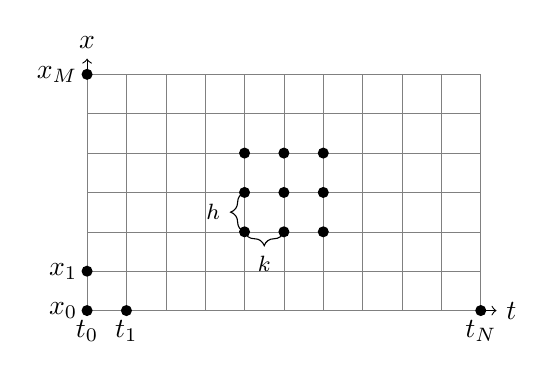
\begin{tikzpicture}

    % Axes
    \draw[->] (0,0) -- (5.2,0) node[right] {\(t\)};
    \draw[->] (0,0) -- (0,3.2) node[above] {\(x\)};

    % Grid points
    \draw[step=0.5cm,gray,very thin] (0,0) grid (5,3);

    \node[below] at (0,0) {\(t_0\)};
    \node[below] at (0.5,0) {\(t_1\)};
    \node[below] at (5,0) {\(t_N\)};
    \node[left] at (0,0) {\(x_0\)};
    \node[left] at (0,0.5) {\(x_1\)};
    \node[left] at (0,3) {\(x_M\)};

    % Add some key points with labels
    \foreach \x in {2,2.5,3} {
        \foreach \y in {1,1.5,2} {
            \fill (\x,\y) circle (2pt);
          }
      }

    % Add curly braces to show length k and h on axes
    \draw [decorate,decoration={brace,amplitude=5pt}]
    (2.5,1) -- (2,1) node [black,midway,yshift=-0.4cm] {\footnotesize \(k\)};
    \draw [decorate,decoration={brace,amplitude=5pt}]
    (2,1) -- (2,1.5) node [black,midway,xshift=-0.4cm] {\footnotesize \(h\)};

    % Add circles/points at nodes
    \fill (0,0) circle (2pt);
    \fill (0.5,0) circle (2pt);
    \fill (5,0) circle (2pt);
    \fill (0,0.5) circle (2pt);
    \fill (0,3) circle (2pt);

  \end{tikzpicture}
\end{center}

\begin{remark}{Constant Grid Spacing}{step_sizes}
  For simplicity, \(h\) and \(k\) are constant \( x_{m+1} = x_m + h,\quad t_{n+1} = t_n + k \).
\end{remark}

\section{Finite Difference Schemes}

Finite difference methods approximate differential equations by replacing them with a system of algebraic equations on the chosen grid.
The heat equation is often solved with these methods for their simplicity and computational efficiency.

\paragraph{The Forward-Time Central-Space (FTCS) scheme}

FTSC is a simple and widely used method for solving the heat equation.
It approximates the time derivative with a forward difference and the spatial derivative with a central difference.


\begin{align*}
  \frac{1}{k} \nabla_t U_m^{n+1} & = \frac{\mu}{h^2} \delta_x^2 U_m^{n+1} + f(U_m^n)                                              \\
  \nabla_t U_m^{n+1}             & = r \delta_x^2 U_m^{n+1} + k f(U_m^n), \quad r = \frac{\mu k}{h^2}                             \\
  U_m^{n+1}                      & = U_m^n + r \left( U_{m+1}^{n+1} - 2 U_m^{n+1} + U_{m-1}^{n+1} \right) + k f(U_m^n) \tag{FTCS}
\end{align*}

\paragraph{Crank-Nicolson Scheme}

The Crank-Nicolson scheme is an implicit method that approximates the spatial derivative at the midpoint between time steps. It is unconditionally stable and second-order accurate in time and space.
\begin{align*}
  U_m^\star & = U_m^n + \frac{r}{2} \left( \delta_x^2 U_m^\star + \delta_x^2 U_m^n \right) + k f(U_m^n), \quad r = \frac{\mu k}{h^2} \\
  U_m^{n+1} & = U_m^\star + \frac{k}{2} \left( f(U_m^\star) - f(U_m^{n+1}) \right) \tag{Crank-Nicolson}
\end{align*}

\section{Error Analysis}
Let \(f(u) = a u\), where \(a\) is a constant.

We denote the exact, and intermediate PDE solution by
\[
  u_m^n = u(x_m, t_n), \quad u_m^\star = u(x_m, t_n + \Phi k)
\]
Where \(\Phi \in [0, 1]\) is a parameter that interpolates between the time levels \(t_n\) and \(t_{n+1}\).

We want to find the local truncation error (LTE) of the Crank-Nicolson scheme, which is the error at a single grid point when approximating the PDE with the finite difference scheme.

\[
  \norm{\tau_m^n} = \norm{u(x_m, t_n) - U_m^n} = \mathcal{O}(h^p + k^q) \quad \text{as} \quad h, k \to 0
\]


\paragraph{Spatial Taylor Expansions}
\begin{align*}
  u_{m+1}^n & \approx u_m^n + h \partial_x u_m^n + \frac{h^2}{2} \partial_x^2 u_m^n + \frac{h^3}{6} \partial_x^3 u_m^n + \mathcal{O}(h^4) \\
  u_{m-1}^n & \approx u_m^n - h \partial_x u_m^n + \frac{h^2}{2} \partial_x^2 u_m^n - \frac{h^3}{6} \partial_x^3 u_m^n + \mathcal{O}(h^4) \\
\end{align*}

\paragraph{Temporal Taylor Expansions}
\begin{align*}
  u_m^{n+1} & \approx u_m^n + k \partial_t u_m^n + \frac{k^2}{2} \partial_t^2 u_m^n + \frac{k^3}{6} \partial_t^3 u_m^n + \mathcal{O}(k^4)                    \\
  u_m^\star & \approx u_m^n + \Phi k \partial_t u_m^n + \frac{(\Phi k)^2}{2} \partial_t^2 u_m^n + \frac{(\Phi k)^3}{6} \partial_t^3 u_m^n + \mathcal{O}(k^4) \\
  &= u_m^n + \Phi k \left( \mu \partial_x^2 u_m^n + a u_m^n \right) + \frac{(\Phi k)^2}{2} \left( \mu \partial_t^2 u_m^n + a \partial_t u_m^n \right) + \mathcal{O}(k^4)
\end{align*}

Then we substitute these expansions into the finite difference schemes to analyze the local truncation error (LTE):

\begin{align*}
  \delta_x^2 u_m^n &= h^2 \partial_x^2 u_m^n + \mathcal{O}(h^4) \\
  \delta_x^2 u_m^\star &= h^2 \partial_x^2 u_m^\star + \mathcal{O}(h^4)\\
  &= h^2 \partial_x^2 \left( u_m^n + \Phi k \partial_t u_m^n + \frac{(\Phi k)^2}{2} \partial_t^2 u_m^n + \mathcal{O}(k^3) \right) + \mathcal{O}(h^4) \\
  &= h^2 \partial_x^2 u_m^n + \Phi k h^2 \partial_x^2 \partial_t u_m^n + \frac{(\Phi k)^2}{2} h^2 \partial_x^2 \partial_t^2 u_m^n + \mathcal{O}(h^4) \\
  &= h^2 \partial_x^2 u_m^n + \Phi k h^2 \partial_x^2 \left( \mu \partial_x^2 u_m^n + a u_m^n \right) + \frac{(\Phi k)^2}{2} h^2 \partial_x^2 \left( \mu \partial_t^2 u_m^n + a \partial_t u_m^n \right) + \mathcal{O}(h^4) \\
\end{align*}

Then in the first step of the Crank-Nicolson scheme, we have
\begin{align*}
  \Delta_{\text{CN1}} &= u_m^\star - \left[u_m^n + \frac{r}{2} \left( \delta_x^2 U_m^\star + \delta_x^2 U_m^n \right) + k a U_m^n\right]\\
  &= \left[ u_m^n + \Phi k \partial_t u_m^n + \frac{(\Phi k)^2}{2} \partial_t^2 u_m^n + \mathcal{O}(k^3) \right] \\
  &\; - \left[ u_m^n + \frac{r}{2} \left( h^2 \partial_x^2 u_m^\star + h^2 \partial_x^2 u_m^n \right) + k a U_m^n \right] \\
  &= \Phi k \partial_t u_m^n + \frac{(\Phi k)^2}{2} \partial_t^2 u_m^n - \frac{r}{2} h^2 \partial_x^2 u_m^\star + \frac{r}{2} h^2 \partial_x^2 u_m^n + \mathcal{O}(h^4 + k^3) \\
\end{align*}
